% load FRI thesis document class with options: 
% - language=english for writing in english as main language [default]
% - language=slovene for writing in slovene as main language
% - funding=logo.pdf for a funded doctoral thesis - doktorska disertacija MR iz gospodarstva, 
% - stage=pre-alpha for early drafts - no chapter thumbs, smaller page size, which leads to increased font sizes when printed on A4 fit to page [seeks for images in directories /img_LQ, /img]
% - stage=alpha for first review by advisor - no chapter thumbs, smaller page size, which leads to increased font sizes when printed on A4 fit to page [seeks for images in directories /img_LQ, /img]
% - stage=beta for seminar 5 - no chapter thumbs, smaller page size, which leads to increased font sizes when printed on A4 fit to page [seeks for images in directories /img_LQ, /img]
% - stage=gamma for senate approval - no chapter thumbs, TODO: includes notes showing reviewer comments (and author response) [seeks for images in directories /img_LQ, /img]
% - stage=gold for final approved version - notes not displayed, chapter pages in colour, chapter thumbs [seeks for images in directories /img_LQ, /img]
% - stage=press for print version - gold with trim marks, includes also coverpage [seeks for images in directories /img_HQ, /img]
\documentclass[language=english,stage=gold]{FRIteza}

\author[A={I Lebar Bajec}]{Iztok Lebar Bajec}

\title[language=english]{Fuzzy model for a computer simulation of bird flocking}
\title[language=slovene]{Mehki model za računalniško simulacijo letenja ptic v jati}

\keywords[language=english]{bird, flock, boid, animat, fuzzy logic, fuzzy modelling, fuzzy animat, artificial life, behavioural animation}
\keywords[language=slovene]{ptica, jata, boid, animat, mehka logika, mehko modeliranje, mehki animat, umetno življenje, vedenjska animacija}

% primer v slovenskem jeziku
%\approvedBy[title={izredni profesor za računalništvo in informatiko}, role={mentor in član ocenjevalne komisije}]{dr. Nikolaj Zimic}
%\approvedBy[title={izredni profesor za računalništvo in informatiko}, role={predsednik ocenjevalne komisije}]{dr. Blaž Zupan}
%\approvedBy[affiliation={University of Rhode Island}, title={Professor Emeritus of Biological Sciences}, role={zunanji član ocenjevalne komisije}]{dr. Frank H. Heppner}
\approvedBy[title={Associate Professor of Computer and Information Science}, role={advisor and examiner}]{dr. Nikolaj Zimic}
\approvedBy[title={Associate Professor of Computer and Information Science}, role={examiner}]{dr. Blaž Zupan}
\approvedBy[affiliation={University of Rhode Island}, title={Professor Emeritus of Biological Sciences}, role={external examiner}]{dr. Frank H. Heppner}

\previousPublication{%
	Lebar~Bajec I, Zimic N, Mraz M (2003) 
	Fuzzifying the thoughts of animats in
	\emph{Fuzzy Sets and Systems: Proceedings of the 10th International Fuzzy Systems Association World Congress (IFSA 2003)}, 
	Lecture Notes in Artificial Intelligence, Vol. 2715,
	eds. Bilgiç T, De~Baets B, Kaynak O. 
	(Springer-Verlag, Berlin), 
	doi:\,\doi{10.1007/3-540-44967-1_23}.
}
\previousPublication{%
	Lebar~Bajec I, Zimic N, Mraz M (2003) 
	Boids with a fuzzy way of thinking, in
	\emph{Proceedings of Artificial Intelligence and Soft Computing (ASC 2003)},
	ed. Leung H.
	(ACTA Press, Anaheim), pp. 58--62.
}
\previousPublication{%
	Lebar~Bajec I (15/04/2005) 
	\emph{Fuzzy logic and bird flock simulations}. 
	Invited lecture, University of Rhode Island, Department of Biological Sciences, Kingston, RI.
}
\previousPublication{%
	Lebar~Bajec I, Zimic N, Mraz M (2005) 
	Simulating flocks on the wing: the fuzzy approach.
	\emph{Journal of Theoretical Biology}
	doi:\,\doi{10.1016/j.jtbi.2004.10.003}.
}

% force correct date display, ignored if stage not gold or press
\forceDate{6}{2005}

% define cover 
% \cover[title=<title to appear on cover page>, loc=<location of the title>, colour=<colour of the title>]{coverImage}
% defaults: title=\title{#}, loc=NE, colour=P1797
% notes:
%  title - use title to insert prefered line breaking with '\\' 
%  loc - options NE, SE, NW, SW
%  colour - options P1797, white, black
\cover[loc={NE}, colour={P1797}]{coverImage.jpg} 
% define spine
% \spine[title=<title to appear on spine>, pages=<number of pages in book>]{thesisId in decimal}
% defaults: title=\title[A={#}], pages=\ztotpages-2
% notes:
%  title - use title to provide a shortended title for the spine 
%  pages - provide the total number of pages in book, excluding cover and jobinfo (number of pages in pdf - 2) 
\spine{80}

% load path for graphics files
%\graphicspath{{img/}}
%\DeclareGraphicsExtensions{.pdf,.png,.jpg} % search order for graphics files

\usepackage{xspace} % helper package for automatic spaces after replacement macros, to be used with caution
%% define common abbreviations
\newcommand{\ie}{i.e.\xspace} % id est ~ that is
\newcommand{\eg}{e.g.\xspace} % exempli gratia ~ for example
\newcommand{\etc}{etc.\xspace} % et cetera ~ and so on
\newcommand{\etal}{\xspace\bbletal\xspace} % et al. ~ and others
\newcommand{\fig}{Fig.} % reference a figure
\newcommand{\figs}{Figs.} % reference multiple figures
\newcommand{\tab}{Tab.} % reference a table

%% define macros for frequently used commands 
\newcommand{\eng}[1]{angl. #1} % english original

%% notation
\newcommand{\R}{\Rset} \newcommand{\Rset}{\ensuremath{\mathbb{R}}} % real numbers symbol
\newcommand{\N}{\Nset} \newcommand{\Nset}{\ensuremath{\mathbb{N}}} % natural numbers symbol
\newcommand{\E}{\Eset} \newcommand{\Eset}{\ensuremath{\mathbb{E}}} % euclidean vector space symbol
\newcommand{\set}[1]{{\ensuremath{\symbfup{#1}}}} % set; introduction + 
\newcommand{\powset}[1]{\ensuremath{\mathcal{P}(#1)}} % power set; introduction +  
\newcommand{\vect}[1]{\ensuremath{\symbfup{#1}}} % vector; introduction + 
\newcommand{\autom}[1]{{\ensuremath{\symrm{#1}}}} % automaton; animat
%
\newcommand{\fset}[1]{{\ensuremath{\tilde{\set{#1}}}}} % fuzzy set; introduction +  
\newcommand{\fpowset}[1]{\ensuremath{\symcal{F}(#1)}} % fuzzy power set; introduction +  
\newcommand{\fautom}[1]{\ensuremath\tilde{\symup{#1}}} % fuzzy automaton; fuzzyanimat
\newcommand{\ffunc}[1]{\ensuremath\tilde{#1}} % fuzzy function; fuzzyanimat
%
\newcommand{\fvar}[1]{\emph{#1}} % fuzzy variable; fuzzymodelling
\newcommand{\kwd}[1]{\textsc{#1}} % keyword; fuzzymodelling
\newcommand{\fval}[1]{\emph{#1}} % fuzzy value; fuzzymodelling
\newcommand{\frule}[1]{\textsc{\MakeLowercase{#1}}} % fuzzy rule; fuzzymodelling
\newcommand{\statement}[1]{\ensuremath\mathscr{#1}} % logical statement; fuzzymodelling
%
\DeclareMathOperator*{\sgn}{sgn} % sign operator; fuzzyanimat
\DeclareMathOperator*{\cog}{cog} % centre of gravity operator; fuzzymodelling
%
\newcommand{\aprod}{\ensuremath\capdot} % algebraic product symbol
%
\newcommand{\fov}{\ensuremath\mathit{fov}} % field of view; \mathit ensures proper kerning between f and o, a common issue for multichar variables

% define additional hyphenation patterns
\sethyphenation{english}{pri-mar-i-ly} % https://www.hyphenation24.com/


\begin{document}

% TODO: show as an example of subfigure use
%\begin{figure}
%	\begin{subfigure}[b]{.5\figurewidth-3.5pt}
%		\noindent\hrulefill\par
%		\includegraphics{fig_fuzzySet_a}
%		\caption{sub A}\label{labA}
%	\end{subfigure}
%	\hfill
%	\begin{subfigure}[b]{.5\figurewidth-3.5pt}
%		\noindent\hrulefill\par
%		\includegraphics{fig_fuzzySet_b}
%		\caption{sub B}\label{labB}
%	\end{subfigure}
%	\caption{Membership functions of a crisp set of real numbers `from 3 to 5' \subref{labA} and a fuzzy set of real numbers `close to 4' \subref{labB}.}
%	\label{fig:fuzzy:set0}
%\end{figure}

\makecoverpage

\frontmatter
 	\maketitle
 	\makeapprovedby
	\makepreviouspublication
 	%signal path for graphics files
\graphicspath{{img/}}





%==============================
\cleardoublepage
\thispagestyle{empty}

\vspace*{55pt}

\begin{centering}

{\textsc{in memoriam}
 \par}

\vspace{.5cm}

{Damjan Oseli 
 \par}

{1975--2004
 \par}

\end{centering}

\vfill






%==============================
\cleardoublepage
\thispagestyle{empty}

\vspace*{55pt}

\begin{centering}

{\setbox0=\hbox{\emph{``Things never turn out the way you think they will.''}}
 \begin{minipage}{\wd0}
 \emph{``Things never turn out the way you think they will.''}\\%[6pt]
 \null \hfill  --- Michael Crichton, \emph{Prey}, 2002.
 \end{minipage}
 \par}

\vspace{.5cm}

{\setbox0=\hbox{\includegraphics{pixar[forTheBirds]}}
 \begin{minipage}{\wd0}
 \includegraphics{pixar[forTheBirds]}\\%[6pt]
 \null \hfill  --- Pixar, \emph{For the Birds}, 2000.
 \end{minipage}
 \par}

\end{centering}

\vfill
\cleardoublepage

 	% !TeX root = ./thesis.tex

% write thesis abstracts
% use \begin{abstract}\end{abstract} for abstract in english
% use \begin{povzetek}\end{povzetek} for abstract in slovene
% note
% with english as primary language the order is povzetek, abstract
% with slovene as primary language the order is abstract, povzetek


%==============================
\begin{povzetek}

%-----
\lipsum[2-4]

\end{povzetek}


%==============================
\begin{abstract}

%-----
\lipsum[2-4]

\end{abstract}

 	% Do thank those that have helped you









%==============================
\begin{acknowledgements}

%-----
Firstly, I wish to thank my thesis advisor, Associate Professor Nikolaj Zimic, without whose support this dissertation would not have been possible. Furthermore, I sincerely thank Assistant Professor Miha Mraz for the long and some times stressing discussions, which always (one way or another) resulted in my moving forward.

My special thanks go to Professor Frank H. Heppner for a prompt response to my e-mail requesting access to his publications and for later generously agreeing to serve as external examiner of my dissertation, despite his busy schedule and the long distance he had to travel.

I thank all members of the Computer Structures and Systems Laboratory who were forced to listen to my discussions related to bird flocks even in such delicate times as coffee breaks.

Last but not least, I wish to thank my beloved Maja for taking her time and reading through the manuscript and correcting all typographical errors and inserting the missing or deleting the misleading commas; TVTB.
\end{acknowledgements}
 	\tableofcontents

\mainmatter
 	% !TeX root = ./thesis.tex


%==============================
\chapter{Introduction}
\label{ch:introduction}
\lipsum[10-11]


%-----
\section{Motivation}
\label{ch:motivation}
\lipsum[12-13]


%----
\section{Scientific Contributions}
\label{ch:contributions}
\lipsum[14-15]


%----
\section{Methodology}
\label{ch:methodology}
\lipsum[16-17]


%----
\section{Dissertation Overview}
\label{ch:overview}
\lipsum[18-19]

 	\input{thesis-ch2_birdflocks}
 	% !TeX root = ./thesis.tex










%==============================
\chapter{The Animat}
\label{ch:animat}


%-----
\section{The Digital Universe}
The first attempts to model artificial life date all the way back to the 1940s. It was then when John von Neumann, while researching advanced computer structures, based on parallel processing, laid the foundations of a special structure denoted as a \emph{cellular automaton}. Indeed, most of the early artificial life research was based on the cellular automaton, Conway's `Game of Life' \cite{gardner:1970} and Langton's self-reproducing loop \cite{langton:1984} being the most renown examples \cite{adami:1998,emmenche:1994,rucker:1993}.

The cellular automaton is formally defined as a \emph{spatial array} of \emph{cells}, where each cell holds a \emph{digital state number} \cite{rucker:1993}. The cells' states are updated in \emph{parallel} at \emph{discrete time steps}. In addition, it is required that the method of updating is \emph{local} and \emph{homogeneous}. In most cases the cells' next states are computed based on their current state and the state of their immediate neighbourhood (\ie\ the states of the cells that are, with respect to their spatial arrangement, adjacent to the observed cell). But the fixed topology of the cellular automaton makes it difficult to apply to modelling the dynamics of organized groups of moving animals. However, according to Mraz \cite{mraz:2000}, the abstract structure that is the most suitable for modelling a cell in the cellular automaton is the Moore automaton \cite{kohavi:1978}.

\begin{definition}
\label{def:Moore}
  The Moore automaton is defined as a five-tuple $\langle\set{X},\set{Q},\set{Y},\delta,\lambda\rangle$, where $\set{X}$, $\set{Q}$ and $\set{Y}$ are non-empty sets representing the input alphabet, the internal states and the output alphabet respectively; $\delta$ is a mapping called the transition function and $\lambda$ is a mapping called the output function:
  \begin{eqnarray}
    & \delta: \set{X}\times \set{Q}\rightarrow \set{Q}, & \\
    & \lambda: \set{Q}\rightarrow \set{Y}. &
  \end{eqnarray}
  At any discrete time step $t \in \set{T}$, where $\set{T}$ is a non-empty set of discrete time steps, the automaton is in a state $q(t) \in \set{Q}$. The state determines its future input-output behaviour. If an input $x(t) \in \set{X}$ is applied, then, in the next discrete time step $t+1$, the automaton assumes a new state $q(t+1) = \delta(x(t),q(t))$ that depends both on the current state and the input. In addition, the automaton emits the output $\lambda(q(t+1)) \in \set{Y}$, which depends on the new state.
\end{definition}

Let me put aside the cellular automaton structure and concentrate on its cell (\ie\ the Moore automaton). In this chapter the Moore automaton shall be extended so that it can be used to represent an inanimate or animate object. The idea of using Moore automata to represent inanimate or animate objects is not new; after all, every artificial life model constructed by using a cellular automaton makes this notion. However, instead of the fixed topology as required by the cellular automaton, a collection of extended Moore automata is not required to be in a fixed spatial arrangement. In other words this means that it can be used to represent the \emph{digital universe} \cite{bentley:2002}. Furthermore, it also means that the objects constituting the digital universe update their states in parallel at discrete time steps and that the method of updating is local yet not necessarily homogeneous.


%-----
\section{The Digital Animal}
\label{sec:animat}
Regardless of the methods used when modelling a digital animal, the basic characteristics of real animals first need to be abstracted. Most people accept or infer that every animal exists in time and space, and is surrounded by inanimate and animate objects (\ie\ the universe). Most people also presume that animals have senses (\ie\ sight, hearing, smell, \etc) through which they have the ability to \emph{perceive} the current state of the universe. An animal is, through \emph{actions} (\eg\ movement), capable of influencing its internal state and the state of the universe. With respect to its current internal state (\eg\ hunger) only certain data from the universe (\eg\ locations of food sources in the vicinity) is important to the animal and its \emph{drive} is to optimize (\eg\ minimize) the rate of their occurrence. The animal selects \emph{actions} (\eg\ feeding) that satisfy its drives. In view of its current internal state and the most pressing drives the animal performs a sequence of muscular movements that will accomplish a combination of these actions (\emph{action selection}). A model that takes into account the above characteristics is commonly referred to as digital (simulated, artificial) animal or \emph{animat} \cite{cliff:1993,watts:1998,wilson:1985}.

Modelling perception, drives and action selection with a Moore automaton is far from being straightforward. To simplify this, the Moore automaton was extended  \cite{lebar_bajec:2002,lebar_bajec:2003a,lebar_bajec:2003b} and the transition function $\delta$ from definition~\ref{def:Moore} reformulated to a three-stage scheme that is presented in \fig~\ref{fig:animat}. As the ideas behind the extension correspond with Wilson's animat \cite{wilson:1985}, I adopted the name and denoted the extended Moore automaton as an animat.

\begin{figure}
  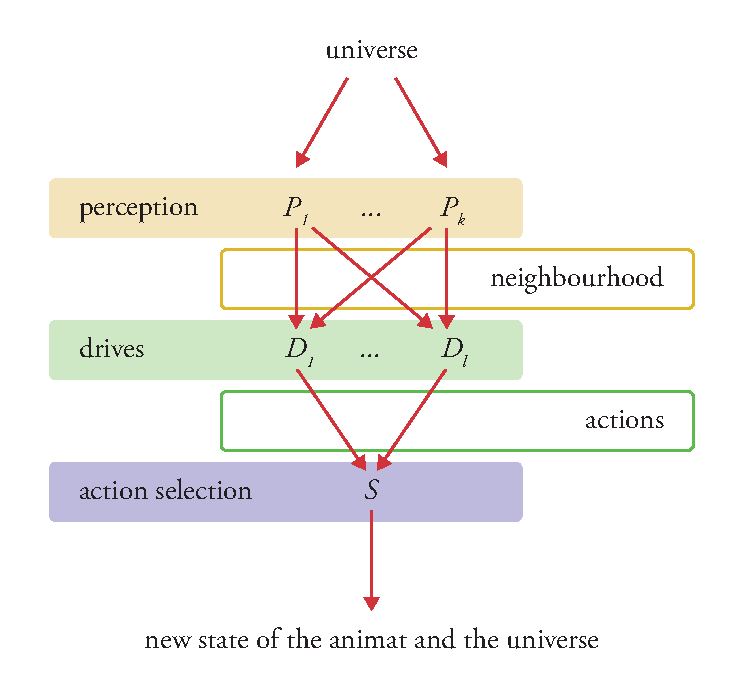
\includegraphics{fig_animat}
  \caption{The animat---the three-stage scheme of the reformulated transition function $\delta$.}
  \label{fig:animat}
\end{figure}

\begin{definition}
  \label{def:animat}
  An animat $\autom{A}=\langle\set{X},\set{Q},\set{Y},\delta,\lambda,P,D,S\rangle$ is an extended Moore automaton, where $P=\langle P_1,\ldots,P_k\rangle$, $D=\langle D_1,\ldots,D_l\rangle$, $S$ are a $k$-tuple of perception functions, an $l$-tuple of drive functions, an action selection function respectively and the transition function $\delta$ is defined as:
  \begin{eqnarray}
    & \delta(x,q) = S(\langle a_1,...,a_l\rangle,q), & \label{eq:animat:delta}\\
    & a_j = D_j(\langle p_1,...,p_k\rangle,q),\ j=1,\ldots,l, & \\
    & p_i = P_i(x,q),\ i=1,\ldots,k. & \label{eq:animat:Pi}
  \end{eqnarray}
\end{definition}

As already said, at the most basic level, the universe is a collection of inanimate and animate objects. I shall assume that it can be represented as a collection of animats (\ie\ extended Moore automata). This means that at a discrete time step $t \in \set{T}$ there are $n(t) \in \N$ animats. Nevertheless, without a loss of generality, it can be assumed that $n(t)=n,\ \forall t \in \set{T}$ and then the animats can be denoted as $\autom{A}_1,\ldots,\autom{A}_n$.

According to the discussion at the beginning of this section, animate and inanimate objects exist in time and space. Let $\E$ be an Euclidean vector space and $\set{S}_i$ represent the set of possible internal states of animal $i$. Then, when modelling organised groups of moving animals, the state of animat $\autom{A}_i$ at a discrete time step $t \in \set{T}$ is typically represented as $q_i(t)=\langle \vect{p}_i(t), \vect{v}_i(t), s_i(t) \rangle$, where $\vect{p}_i(t) \in \E$ denotes the position in space, $\vect{v}_i(t) \in \E$ the velocity and $s_i(t) \in \set{S}_i$ the internal state of the modelled animal.

Let $\set{Y}_i$ denote the output alphabet of animat $\autom{A}_i$ for all $i=1,\ldots,n$. It is a non-empty set representing data about animal $i$ that can be perceived by an outside observer. Therefore $\set{U}=\set{Y}_1 \times \cdots \times \set{Y}_n$ and the perceivable state of the universe at a discrete time step $t \in \set{T}$ is given by the $n$-tuple $u(t)=\langle y_1(t),\ldots,y_n(t)\rangle$, where $y_i(t)=\lambda_i(q_i(t))$ denotes the output of animat $\autom{A}_i$ at time step $t$ for all $i=1,\ldots,n$.

At any discrete time step all animats are applied the same input; the perceivable state of the universe. In other words, at a discrete time step $t \in \set{T}$, the input that is applied to all animats is $x(t)=u(t)$. Subsequently this means that all animats use the input alphabet $\set{X}=\set{U}=\set{Y}_1 \times \cdots \times \set{Y}_n$.

If I summarize: at a discrete time step an animat is applied the current perceivable state of the universe (\ie\ the data about all of the animats that can be perceived by an outside observer). Using the transition function (\ie\ taking into consideration perception, drives and action selection), the animat computes its next discrete time step state and then emits its new output. With this the perceivable state of the universe changes. In the following sections perception, drives and action selection are going to be discussed in more detail.

%--
\subsection{Perception}
As already said, the input of an animat is the current perceivable state of the universe. Let perception be the animal's process of \emph{interpreting} the perceivable data and \emph{selecting} just the relevant information from all of the sensory signals that exist in the universe (\eg\ detect the locations of food sources in the vicinity). From the viewpoint of human perception of the universe, it could be said that there exist multiple perception types (\ie\ sight, hearing, smell, \etc), where each of them selects only the relevant information according to a specific characteristic.

Let the current perceivable state of the universe be the $n$-tuple  $u=\langle y_1,\ldots,y_n\rangle$, where for all $i=1,\ldots,n$ $y_i \in \set{Y}_i$ is data about animat $\autom{A}_i$ that can be perceived by an outside observer. Let $q \in \set{Q}$ be the current state of the observed animat and let its input $x \in \set{X}$ be the current perceivable state of the universe, that is  $x=u=\langle y_1,\ldots,y_n \rangle$.

Let $\N_n$ denote the set of all positive natural numbers lower or equal to $n$ and for all $i=1,\ldots,n$ let the set $\set{I}^\textnormal{c}_i$ represent information about animat $\autom{A}_i$ that can be obtained from $y_i$ with respect to a certain characteristic $\mathrm{c}$.

Let the set $\set{N} \in \powset{\N_n}$ represent the set of indexes of members of $x$; in other words, animats that are according to characteristic $\mathrm{c}$ relevant to the observed animat. The ordered pair $p=\langle\set{N},o\rangle$, where $\set{N} \in \powset{\N_n}$ and $o \in \set{I}^\textnormal{c}_1 \times \cdots \times \set{I}^\textnormal{c}_n$ then represents the information regarding characteristic $\textnormal{c}$ that was obtained from the current perceivable state of the universe and is, with respect to this characteristic, relevant to the observed animat. For reasons of notational simplicity, let the set $\powset{\N_n} \times (\set{I}^\textnormal{c}_1 \times \cdots \times \set{I}^\textnormal{c}_n)$ be denoted simply as $\set{P}^\textnormal{c}$.

\begin{definition}
  \label{def:animat:Pi}
  Let $x \in \set{X}$ be the current perceivable state of the universe and $p \in \set{P}^\textnormal{c}$ be the information regarding characteristic $\mathrm{c}$ that was obtained from $x$ and is, according to this characteristic and the state $q \in \set{Q}$, relevant to the animat. Then a \emph{perception function} for characteristic $\mathrm{c}$ is a mapping $P: \set{X} \times \set{Q} \mapsto \set{P}^\textnormal{c}$.
\end{definition}

For reasons of simplicity I shall address the image of a perception function with the name \emph{neighbourhood}. If I sum up, a neighbourhood obtained by means of a perception function represents only the relevant characterized sensory signals (\eg\ locations of food sources in the vicinity). This means that the perception function allows taking into account that different animals employ different strategies for sampling sensory data \cite{cliff:1993}.

%--
\subsection{Drives}
The animal's drives are in strong correlation of its internal state and the perceived information about the state of the universe. In other words: based on the information obtained from the perceivable state of the universe (\eg\ locations of food sources in the vicinity) and its current internal state (\eg\ hunger) the animal will select actions (\eg\ feeding) that satisfy a specific \emph{drive} (\eg\ minimize hunger).

Let the observed animat have $k \in \N$ perception functions denoted as $P_1,\ldots,P_k$. This means that the set $\set{P}=\set{P}^{\mathrm{c}_1} \times \cdots \times \set{P}^{\mathrm{c}_k}$ represents information obtainable from the perceivable state of the universe. Let me for all $i=1,\ldots,k$ use $p_i \in  \set{P}^{\mathrm{c}_i}$ to denote the neighbourhood that was obtained using perception function $P_i$. Then $\langle p_1,\ldots,p_k\rangle \in \set{P}$ represents the perceived information about the current state of the universe that was, with respect to the current state of the animat, obtained from the current perceivable state of the universe.

\begin{definition}
  \label{def:animat:Dj}
  Let $\set{A}$ denote the set of possible actions of the animat and let $a \in \set{A}$ be the action that, with respect to the perceived information about the current state of the universe $\langle p_1,\ldots,p_k\rangle \in \set{P}$ and the current state of the animat $q \in \set{Q}$, satisfies a specific drive. Then a \emph{drive function} is a mapping $D: \set{P} \times \set{Q} \mapsto \set{A}$.
\end{definition}

%--
\subsection{Action Selection}
With action selection I refer to the animal's neurological process of \emph{selecting} the \emph{sequence of muscular movements} that will accomplish the actions that result from its drives. This process must combine, prioritize, and arbitrate between potentially conflicting actions.

Let the observed animat have $l \in \N$ drive functions denoted as $D_1,\ldots,D_l$. This means that the $l$-tuple $\langle a_1,\ldots,a_l\rangle \in \set{A}^l$ represents the animat's desired actions (\ie\ the actions that would satisfy its drives, each satisfying only one of them).

\begin{definition}
  \label{def:animat:S}
  Let $q' \in \set{Q}$ denote the next state of the animat computed by taking into account the current state of the animat $q \in \set{Q}$ and combining, prioritizing and arbitrating between its desired actions $\langle a_1,\ldots,a_l\rangle \in \set{A}^l$. Then an \emph{action selection function} is a mapping $S: \set{A}^l \times \set{Q} \rightarrow \set{Q}$.
\end{definition}

If I sum up, at any discrete time step the animat's input is the current state of the universe. The three stage scheme of the transition function, given by equations~\eqref{eq:animat:delta}--\eqref{eq:animat:Pi}, tries to imitate the adopted theory about the behaviour of animals (\fig~\ref{fig:animat}). In the first stage the perception functions are used to retrieve, from the current perceivable state of the universe, only the information that is relevant to the observed animat. In the second stage the drive functions use the retrieved information to compute the desired actions (\ie\ those that would satisfy the observed animat's drives). Finally the action selection function combines, prioritizes and arbitrates between the potentially conflicting actions and generates the animat's next discrete time step state.

%-----
\section{Case Study}
In the previous sections a formal definition of the animat was  presented. The animat can be used to model an inanimate or animate object. In this section I shall employ it to reproduce the computer models of bird flocking that were presented by Reynolds \cite{reynolds:1987} and Heppner and Grenander \cite{heppner:1990}. This way I will show the usability of the animat and also present the formalization of the two models.

Reynolds based all of his processing on geometrical calculations, but even though he has published numerous works concerning his model \cite{reynolds:1987,reynolds:1993a,reynolds:1993b,reynolds:1994,reynolds:1999,reynolds:2000}, no formal definitions have ever been given. Fortunately, he has recently made available the OpenSteer library,\footnote{\href{http://opensteer.sourceforge.net}{http://opensteer.sourceforge.net}} which includes an implementation of the model. Therefore all of my studies are based on this implementation, more precisely on OpenSteer v0.8.

Heppner and Grenander, on the other hand, based their processing on stochastic differential equations. In their paper, as a contrast to Reynolds's, they give more information, but which is not sufficiently complete to allow for an immediate easy reimplementation. Furthermore, the model they used is not available on-line. Recently, however, Heppner has given me a printout of the source code of the model through personal correspondence, and thus I have based my studies on the latter.

%--
\subsection{Formalization of Reynolds's Computer Model}
\label{subsec:animat:cwr}
Reynolds in his study \cite{reynolds:1987} modelled the universe as a collection of $n$ digital birds of the same kind and obstacles which represented inanimate objects. He states that the obstacles and the digital birds' attempts to navigate around them increase the apparent complexity of the displayed behaviour. In his paper he also suggests that the complexity of natural flocks might be due largely to the complexity of the natural environment \cite{reynolds:1987}. More recently,\footnote{\href{http://www.red3d.com/cwr/boids/applet/}{http://www.red3d.com/cwr/boids/applet/}} however, he has acknowledged that the lifelike, unpredictable behaviour of the digital birds emerges from the complex adaptive nature of the model. Furthermore, in his latest studies \cite{reynolds:1999,reynolds:2000} he states that flock-like behaviour can be achieved by using only three drives and is independent of obstacles. Thus I decided not to model the obstacles, after all, natural flocks form and exist even in open spaces, where there are no obstacles.

As already said, Reynolds's digital bird moves through the universe with a certain velocity (\ie\ flight direction and flight speed) and at every discrete time step it changes this velocity in order to approximately optimize three drives: \emph{separation}, \emph{alignment}, and \emph{cohesion} (see subsection~\ref{subsec:birdFlocks:cwr}). The decision is based purely on the digital bird's current state and the current perceivable state of the universe. More precisely, the decision is based on the perceived locations and velocities of the nearby flockmates. However, the meaning of the expression `nearby flockmates' is drive dependant. Regardless of the latter, the above led me to believe that Reynolds's digital bird could be represented as an animat \cite{lebar_bajec:2002,lebar_bajec:2003a,lebar_bajec:2003b}.

I shall assume that Reynolds's digital bird can be represented as an animat. As discussed in section~\ref{sec:animat}, the animat's internal state $q \in \set{Q}$ is defined by the triplet $\langle\vect{p},\vect{v},s\rangle$, where $\vect{p} \in \E$ is its position in space, $\vect{v} \in \E$ its velocity and $s \in \set{S}$ is the modelled animal's internal state. I shall therefore begin by defining the latter.

\begin{definition}
  \label{def:animat:s:cwr}
  Let the triplet $r=\langle r_\textnormal{s}, r_\textnormal{a}, r_\textnormal{c}\rangle$ represent the separation, alignment and cohesion perception distances and let the triplet $\fov=\langle\fov_\textnormal{s}, \fov_\textnormal{a}, \fov_\textnormal{c}\rangle$ represent the separation, alignment and cohesion fields of view. Let $m$ represent the digital bird's mass, $v_\textnormal{M}$ its maximal achievable flight speed and $f_\textnormal{M}$ its maximal available force. Then the internal state of the animal modelled by Reynolds's digital bird is
  \begin{equation}
  s=\langle \mathrm{r}, \fov, m, v_\textnormal{M}, f_\textnormal{M} \rangle.
  \end{equation}
\end{definition}

For reasons of simplicity it shall be assumed that only the animat's position $\vect{p}$ and velocity $\vect{v}$ change through time, while the modelled animal's internal state $s$ stays constant. This is also consistent with Reynolds's original definition \cite{reynolds:1987}. The velocity vector $\vect{v}$ gives the animat's relative position changes per coordinate axis in the Cartesian coordinate system and therefore encodes the animat's flight direction $\vect{v}^0$ and flight speed $\left\|\vect{v}\right\|$. The perception distances and fields of view define the animal's perception volume (\fig~\ref{fig:perception:cwr}). The maximal achievable speed represents a simple model of viscous speed damping (\ie\ it will be used to model the inability to exceed a certain speed even if constantly accelerating), while the maximal available force shall be used to take into account the fact that only an animal with a finite amount of energy is being modelled.

\begin{figure}
  \includegraphics{fig_perception_cwr}
  \caption{The perception model that Reynolds used in the OpenSteer v0.8 implementation of his model \cite{reynolds:1999}. The black arrow represents the digital bird's flight direction. The shaded area represents the combined perception volume defined by the distinct separation ($r_\textnormal{s}$,$\fov_\textnormal{s}$), alignment ($r_\textnormal{a}$,$\fov_\textnormal{a}$) and cohesion ($r_\textnormal{c}$,$\fov_\textnormal{c}$) perception volumes. The perceived flockmates are depicted in a light blue colour.}
  \label{fig:perception:cwr}
\end{figure}

%-
\subsubsection{Modelling Perception}
As discussed before, in Reynolds's case, the universe is homogeneous (\ie\ consists of animats of the same kind). Furthermore, the number of animats is $n \in \N$ and constant through time. This means that the animat's input alphabet is $\set{X}=\set{Y}^n$.

Let $\set{Y}=\E \times \E$ and let the animat's output function $\lambda(q)=\langle\vect{p},\vect{v}\rangle$ return the animat's current position in space and its current velocity. Then at a discrete time step $t \in \set{T}$ the perceivable state of the universe is $u(t)=\langle y_1(t),\ldots,y_n(t)\rangle$, where for all $i=1,\ldots,n$ $y_i(t)=\lambda(q_i(t))$ is the output of animat $i$ (\ie\ its position in space and its velocity) at time step $t$.

As said, a perception function (definition~\ref{def:animat:Pi}) acts like an interpreter of the perceivable state of the universe and a selector of relevant information. Then, regarding the drives employed by Reynolds and the OpenSteer v0.8 source code, three perception functions $P_\textnormal{s}$, $P_\textnormal{a}$ and $P_\textnormal{c}$ must be defined. The separation perception function $P_\textnormal{s}$ returns the locations of the flockmates that must be avoided, the alignment perception function $P_\textnormal{a}$ returns the velocities of flockmates that should be followed and the cohesion perception function $P_\textnormal{c}$ returns the locations of flockmates that should be kept close to.

Let $\autom{B}_i$ and $\autom{B}_j$, where $i,j \in \N_n$, be two animats from Reynolds's digital universe and let $q_j=\langle\vect{p}_j,\vect{v}_j,s_j\rangle$ be the current state of animat $\autom{B}_j$ and $y_i=\lambda(q_i)=\langle \vect{p}_i,\vect{v}_i \rangle$ be the current output of animat $\autom{B}_i$ (\ie\ the perceivable data about it). Let $\autom{B}_j$ denote the observed animat. Then the distance of animat $\autom{B}_i$ is computed as
%
\begin{equation}
  \varepsilon_i=\left\|\vect{p}_i - \vect{p}_j\right\|, \label{eq:animat:cwr:distance}
\end{equation}
%
and the direction of the offset vector between them is computed as
%
\begin{equation}
  \varphi_i=\arccos \left( \frac {\vect{v}_j \cdot (\vect{p}_i - \vect{p}_j)}{\left\| \vect{v}_j \right\| \left\| \vect{p}_i - \vect{p}_j \right\|} \right). \label{eq:animat:cwr:angularOffset}
\end{equation}

\begin{definition}
  \label{def:animat:Ps:cwr}
  Let $x=\langle y_1,\ldots,y_n\rangle$ be the current perceivable state of the universe and $j$ the index of the observed animat. Let $\set{I}^\textnormal{s}=\E$ be the set representing obtainable information about a flockmate's location. Then $\set{P}^\textnormal{s}=\powset{\N_n} \times \E^n$ and equations~\eqref{eq:animat:Ps0:cwr}--\eqref{eq:animat:Ps2:cwr} define the \emph{separation perception function} $P_\textnormal{s}: \set{X} \times \set{Q} \mapsto \set{P}^\textnormal{s}$.
  \begin{eqnarray}
    & P_\textnormal{s}(x,q)=\langle\set{N}_\textnormal{s},o_\textnormal{s}\rangle, & \label{eq:animat:Ps0:cwr} \\
    & \set{N}_\textnormal{s}=\left\{i|\ i \in \N_n,\ i \neq j,\ \varepsilon_i%(q,y_i)
     \leq r_\textnormal{s},\ \varphi_i%(q,y_i)
     < \fov_\textnormal{s} \right\}, & \\
    & o_\textnormal{s}=\langle \vect{p}_1,\ldots,\vect{p}_n\rangle. & \label{eq:animat:Ps2:cwr}
  \end{eqnarray}
\end{definition}

\begin{definition}
  \label{def:animat:Pa:cwr}
  Let $x=\langle y_1,\ldots,y_n \rangle$ be the current perceivable state of the universe and $j$ the index of the observed animat. Let $\set{I}^\textnormal{a}=\E$ be the set representing obtainable information about a flockmate's velocity. Then $\set{P}^\textnormal{a}=\powset{\N_n} \times \E^n$ and equations~\eqref{eq:animat:Pa0:cwr}--\eqref{eq:animat:Pa2:cwr} define the \emph{alignment perception function} $P_\textnormal{a}: \set{X} \times \set{Q} \mapsto \set{P}^\textnormal{a}$.
  \begin{eqnarray}
    & P_\textnormal{a}(x,q)=\langle\set{N}_\textnormal{a},o_\textnormal{a}\rangle, & \label{eq:animat:Pa0:cwr} \\
    & \set{N}_\textnormal{a}=\left\{i|\ i \in \N_n,\ i \neq j,\ \varepsilon_i%(q,y_i)
     \leq r_\textnormal{a},\ \varphi_i%(q,y_i)
     < \fov_\textnormal{a}\right\}, & \\
    & o_\textnormal{a}=\langle \vect{v}_1,\ldots,\vect{v}_n\rangle. & \label{eq:animat:Pa2:cwr}
  \end{eqnarray}
\end{definition}

\begin{definition}
  \label{def:animat:Pc:cwr}
  Let $x=\langle y_1,\ldots,y_n \rangle$ be the current perceivable state of the universe and $j$ the index of the observed animat. Let $\set{I}^\textnormal{c}=\E$ be the set representing obtainable information about a flockmate's location. Then $\set{P}^\textnormal{c}=\powset{\N_n} \times \E^n$ and equations~\eqref{eq:animat:Pc0:cwr}--\eqref{eq:animat:Pc2:cwr} define the \emph{cohesion perception function} $P_\textnormal{c}: \set{X} \times \set{Q} \mapsto \set{P}^\textnormal{c}$.
  \begin{eqnarray}
    & P_\textnormal{c}(x,q)=\langle\set{N}_\textnormal{c},o_\textnormal{c}\rangle, & \label{eq:animat:Pc0:cwr} \\
    & \set{N}_\textnormal{c}=\left\{i|\ i \in \N_n,\ i \neq j,\ \varepsilon_i%(q,y_i)
     \leq r_\textnormal{c},\ \varphi_i%(q,y_i)
     < \fov_\textnormal{c}\right\}, & \\
    & o_\textnormal{c}=\langle \vect{p}_1,\ldots,\vect{p}_n\rangle. & \label{eq:animat:Pc2:cwr}
  \end{eqnarray}
\end{definition}

To sum up, the three perception functions together return only those digital birds that are in the perception volume of the observed digital bird. In other words, each of the three neighbourhoods represents only the flockmates that are treated as `nearby' according to the digital bird's corresponding drive \cite{reynolds:1987} (see subsection~\ref{subsec:birdFlocks:cwr}).

%-
\subsubsection{Modelling Drives}
Recall that a drive function (definition~\ref{def:animat:Dj}), based on the current perceived information about the state of the universe and the current state of the animat, selects the action to satisfy a specific drive. Then, since Reynolds states that flock-like behaviour can be achieved if the digital bird follows three drives, three drive functions $D_\textnormal{s}$, $D_\textnormal{a}$ and $D_\textnormal{c}$ need to be defined. The separation drive function $D_\textnormal{s}$ returns the action that will keep the animat safe from colliding with the flockmates which should be avoided. The alignment drive function $D_\textnormal{a}$ returns the action that will align it with the flockmates which should be followed and the cohesion drive function $D_\textnormal{c}$ returns the action that will direct it towards the centre of the flockmates which should be kept close to. Reynolds models the drives using geometrical equations (detailed descriptions are presented in \cite{reynolds:1999}) and since he models the digital bird as a simple vehicle \cite{reynolds:1987,reynolds:1999}, he represents the desired actions as physical forces which would induce the desired flight direction and/or flight speed change.

Let the animat's $k$-tuple of perception functions be  $P=\langle P_\textnormal{s},P_\textnormal{a},P_\textnormal{c}\rangle$. Then, according to definition~\ref{def:animat:Dj} and definitions~\ref{def:animat:Ps:cwr}--\ref{def:animat:Pc:cwr}, the set representing information obtainable from the perceivable state of the universe is $\set{P}=\set{P}^\textnormal{s} \times \set{P}^\textnormal{a} \times \set{P}^\textnormal{c}$.

According to Reynolds \cite{reynolds:1999}, the separation drive gives the digital bird the ability to maintain a certain separation distance from nearby flockmates. In this case the nearby flockmates are the digital birds that should be avoided (\ie\ computed using the separation perception function). For each flockmate a `repulsive force' is computed by subtracting the current position of the observed animat and the current position of the flockmate. This force is then divided by the square of the flockmate's distance.\footnote{Reynolds admits \cite{reynolds:1999} that the division by the square of the flockmate's distance is just a setting that worked well and not a fundamental value.} The resulting forces are then summed together, and according to \sidenote{OpenSteer v0.8}{!animats v1.0 should first average then normalize---opensteer does so!} also normalized, to produce the desired action (\ie\ the desired change in flight direction and flight speed).

\begin{definition}
  \label{def:animat:Ds:cwr}
  Let the current state of the animat be $q=\langle\vect{p},\vect{v},s\rangle$. Let the information that was, with respect to the current state of the animat $q$, obtained from the current perceivable state of the universe be $\langle p_\textnormal{s},p_\textnormal{a},p_\textnormal{c}\rangle \in \set{P}$ and let $p_\textnormal{s}=\langle\set{N}_\textnormal{s},o_\textnormal{s}\rangle$, where $\set{N}_\textnormal{s} \in \powset{\N_n}$ is a set representing the indexes of animats that should be avoided and $o_\textnormal{s}=\langle\vect{p}_1,\ldots,\vect{p}_n\rangle$ are their current positions in space. Let the set of available actions be $\set{A}=\E$. The \emph{separation drive function} is then the drive function $D_\textnormal{s}: \set{P} \times \set{Q} \mapsto \set{A}$ that is defined as
  \begin{equation}
    D_\textnormal{s}(\langle p_\textnormal{s},p_\textnormal{a},p_\textnormal{c}\rangle, q) = \left[ \sum_{i \in \set{N}_\textnormal{s}} \frac{\vect{p}-\vect{p}_i}{{\left\|\vect{p}_i-\vect{p}\right\|}^2} \right]^0. \label{eq:animat:Ds:cwr}
  \end{equation}
\end{definition}

The alignment drive, on the other hand, gives the digital bird the ability to align itself with (\ie\ fly in the same flight direction and/or with the same speed as) the nearby flockmates. The nearby flockmates in this case are the digital birds that should be followed. The average of the velocities of these flockmates is computed and represents the desired new velocity of the observed digital bird. The velocity difference is computed by subtracting the observed digital bird's velocity from the desired new velocity. Finally the force representing the desired action is then, according to OpenSteer v0.8, computed by normalizing the velocity difference.

\begin{definition}
  \label{def:animat:Da:cwr}
  Let the current state of the animat be $q=\langle\vect{p},\vect{v},s\rangle$. Let the information that was, with respect to the current state of the animat $q$, obtained from the current perceivable state of the universe be $\langle p_\textnormal{s},p_\textnormal{a},p_\textnormal{c}\rangle \in \set{P}$ and let $p_\textnormal{a}=\langle\set{N}_\textnormal{a},o_\textnormal{a}\rangle$, where $\set{N}_\textnormal{a} \in \powset{\N_n}$ is a set representing the indexes of animats that should be followed and $o_\textnormal{a}=\langle\vect{v}_1,\ldots,\vect{v}_n\rangle$ are their current velocities. Let the set of available actions be $\set{A}=\E$. The \emph{alignment drive function} is then the drive function $D_\textnormal{a}: \set{P} \times \set{Q} \mapsto \set{A}$ that is defined as
  \begin{equation}
    D_\textnormal{a}(\langle p_\textnormal{s},p_\textnormal{a},p_\textnormal{c}\rangle, q) = \left[ \Biggl( \frac{1}{\left|\set{N}_\textnormal{a}\right|} \sum_{i \in \set{N}_\textnormal{a}} \vect{v}_i \Biggr) - \vect{v} \right]^0. \label{eq:animat:Da:cwr}
  \end{equation}
\end{definition}

Finally, the cohesion drive gives the digital bird the ability to cohere with (\ie\ approach and form a group with) the nearby flockmates. Here the nearby flockmates are the digital birds that should be kept close to. The centre (\ie\ the \emph{centre of mass} or \emph{average position}) of these flockmates is computed and represents the desired position of the observed digital bird. The `attraction force' is computed by subtracting the observed digital bird's position from the desired position. At last the force representing the desired action is, according to OpenSteer v0.8, computed by normalizing the attraction force.

\begin{definition}
  \label{def:animat:Dc:cwr}
  Let the current state of the animat be $q=\langle\vect{p},\vect{v},s\rangle$. Let the information that was, with respect to the current state of the animat $q$, obtained from the current perceivable state of the universe be $\langle p_\textnormal{s},p_\textnormal{a},p_\textnormal{c}\rangle \in \set{P}$ and let $p_\textnormal{c}=\langle\set{N}_\textnormal{c},o_\textnormal{c}\rangle$, where $\set{N}_\textnormal{c} \in \powset{\N_n}$ is a set representing the indexes of animats that should be kept close to and $o_\textnormal{c}=\langle\vect{p}_1,\ldots,\vect{p}_n\rangle$ are their current positions in space. Let the set of available actions be $\set{A}=\E$. The \emph{cohesion drive function} is then the drive function $D_\textnormal{c}: \set{P} \times \set{Q} \mapsto \set{A}$ that is defined as
  \begin{equation}
    D_\textnormal{c}(\langle p_\textnormal{s},p_\textnormal{a},p_\textnormal{c}\rangle, q) = \left[ \left( \frac{1}{\left|\set{N}_\textnormal{c}\right|} \sum_{i \in \set{N}_\textnormal{c}} \vect{p}_i \right) - \vect{p} \right]^0. \label{eq:animat:Dc:cwr}
  \end{equation}
\end{definition}

%-
\subsubsection{Modelling Action Selection}
Each of the three drive functions returns a physical force that would satisfy the specific drive. Recall that the action selection function (definition~\ref{def:animat:S}), combines, prioritizes and arbitrates between potentially conflicting actions to select the sequence of muscular movements that will eventually accomplish all of the animal's drives. In his original study Reynolds \cite{reynolds:1987} proposes that the physical forces should be combined using a special algorithm named \emph{prioritized acceleration allocation}. But in one of his later studies \cite{reynolds:1999} he also admits that in the course of several reimplementations of the model over the years, a simpler linear combination has proved sufficient. Moreover, in his latest implementation in OpenSteer v0.8 he uses a weighted sum combination.

This means that Reynolds models action selection as a weighted sum of the desired actions (\ie\ weighted sum of the respective physical forces). The resulting force is used to compute the digital bird's new position in space and velocity. This computation is subjected to a set of constraints modelling conservation of momentum, viscous damping and the animal's finite amount of energy. He names the approach \emph{geometrical flight} \cite{reynolds:1987}.

\sidenote{Reynolds does not model the musculoskeletal structure of a bird}{v1.1.20050210 [FHH]: this may be a very unrealistic assumption---birds, like air planes, have stability-producing features that make them tend to go in a straight line unless positively directed otherwise.\\v1.3.20050402 [ILB]: This is taken care of by geometrical flight.}, but models it as a point mass vehicle \cite{reynolds:1987,reynolds:1999}. This means that the animat's physics is based on forward Euler integration. In other words, the combined forces (limited by the animat's maximal available force) are applied to the animat's point mass. This produces an acceleration equal to the combined force divided by the animat's mass. The acceleration is then added to the animat's current velocity and truncated by the maximum achievable speed. Finally the animat's new position in space is computed by adding the new velocity to the animat's current position in space.

Let $\vect{a} \in \E$ be a vector and let $a \in \R^+$ represent the maximal size of $\vect{a}$. Then the truncation of vector $\vect{a}$ to its maximal size $a$ is calculated as
%
\begin{equation}
  \lfloor\vect{a}\rceil^{a} = \min(\left\|\vect{a}\right\|, a) \vect{a}^0. \label{eq:truncation}
\end{equation}

\begin{definition}
  \label{def:animat:Sws:cwr}
  Let the current state of the animat be $q=\langle\vect{p},\vect{v},s\rangle$, where the modelled animal's internal state $s$ is defined by definition~\ref{def:animat:s:cwr}. Let the $l$-tuple of drive functions be $D=\langle D_\textnormal{s}, D_\textnormal{a}, D_\textnormal{c}\rangle$ and let the computed desired actions be $\langle a_\textnormal{s},a_\textnormal{a},a_\textnormal{c}\rangle$. Let $w_\textnormal{s}$, $w_\textnormal{a}$ and $w_\textnormal{c}$ represent the weights of the separation, alignment and cohesion drive respectively and let $dt$ represent the simulation step. Then the \emph{weighted sum action selection function} is the action selection function $S_\textnormal{ws}: \set{A} \times \set{Q} \mapsto \set{Q}$ that is defined as
  \begin{equation}
    S_\textnormal{ws}(\langle a_\textnormal{s},a_\textnormal{a},a_\textnormal{c}\rangle, q) = \langle\vect{p}', \vect{v}', s\rangle, \label{eq:animat:Sws0:cwr}
  \end{equation}
  \vspace{-3mm}
  \begin{equation}
    \vect{v}' = \left\lfloor {\vect{v} + \frac{\left\lfloor w_\textnormal{s}a_\textnormal{s} + w_\textnormal{a}a_\textnormal{a} + w_\textnormal{c}a_\textnormal{c} \right\rceil^{f_\textnormal{M}}}{m}}dt \right\rceil^{v_\textnormal{M}},
  \end{equation}
  \vspace{-3mm}
  \begin{equation}
    \vect{p}' = \vect{p} + \vect{v}'dt. \label{eq:animat:Sws2:cwr}
  \end{equation}
\end{definition}

Therefore Reynolds's digital bird can be defined as a special animat.

\begin{definition}
  \label{def:animat:cwr}
  Reynolds's digital bird is the animat $\autom{B}=\langle\set{X},\set{Q},\set{Y},\delta,\lambda,P,D,S\rangle$. The set representing internal states is $\set{Q}=\E \times \E \times \set{S}$, where $\set{S}$ is defined by definition~\ref{def:animat:s:cwr}. The output alphabet is $\set{Y}=\E \times \E$ and the input alphabet is $\set{X}=\set{Y}^n$. The animat's current internal state $q=\langle\vect{p},\vect{v},s\rangle$ represents the modelled animal's current position in space $\vect{p} \in \E$, velocity $\vect{v} \in \E$ and internal state $s \in \set{S}$. The output function $\lambda: \set{Q} \mapsto \set{Y}$ is $\lambda(q)=\langle\vect{p},\vect{v}\rangle$. The $k$-tuple of perception functions is $P=\langle P_\textnormal{s},P_\textnormal{a},P_\textnormal{c}\rangle$, where $P_\textnormal{s}$, $P_\textnormal{a}$ and $P_\textnormal{c}$ are the separation, alignment and cohesion perception function respectively (definitions~\ref{def:animat:Ps:cwr}--\ref{def:animat:Pa:cwr}). The $l$-tuple of drive functions is $D=\langle D_\textnormal{s},D_\textnormal{a},D_\textnormal{c}\rangle$, where $D_\textnormal{s}$, $D_\textnormal{a}$ and $D_\textnormal{c}$ are the separation, alignment and cohesion drive function respectively (definitions~\ref{def:animat:Ds:cwr}--\ref{def:animat:Dc:cwr}). Finally, the action selection function is the weighted sum action selection function $S=S_\textnormal{ws}$ (definition~\ref{def:animat:Sws:cwr}).
\end{definition}

%--
\subsection{Formalization of Heppner and Grenander's Computer Model}
\label{subsec:animat:fhh}
Heppner and Grenander in their study \cite{heppner:1990} modelled the universe as a collection of $n$ digital birds of the same kind. As a contrast to Reynolds they did not model any obstacles, but added a special influence modelling random distractions. Furthermore, they admit that without this influence they were not able to achieve flock-like behaviour.

Nevertheless, all things considered, they had a similar approach as Reynolds. Their digital bird moves through the universe with a certain velocity and at every discrete time step it changes this velocity in order to satisfy three drives: \emph{homing}, \emph{velocity regulation}, and \emph{interaction} (see subsection~\ref{subsec:birdFlocks:fhh}). The decision is again based purely on the digital bird's current state and the current perceivable state of the universe. More precisely the decision is based on the digital bird's position, velocity and the perceived locations of the nearby flockmates.

Let me define the animat that models Heppner and Grenander's digital bird. As discussed in section~\ref{sec:animat}, the animat's internal state $q \in \set{Q}$ is defined by the triplet $\langle \vect{p}, \vect{v}, s \rangle$, where $\vect{p} \in \E$ is its position in space, $\vect{v} \in \E$ its velocity and $s \in \set{S}$ is the modelled animal's internal state. Let me again first define the latter.

\begin{definition}
  \label{def:animat:s:fhh}
  Let $\vect{r} \in \E$ be the position of the centre of the roosting area of the the modelled bird, $r_\textnormal{o}$ its perception range, $v_\textnormal{p}$ its preferred flight speed and $d_\textnormal{p}$ its preferred distance from flockmates. Then the internal state of the animal modelled by Heppner and Grenander's digital bird is
  \begin{equation}
    s=\langle \vect{r}, r_\textnormal{o}, v_\textnormal{p}, d_\textnormal{p} \rangle.
  \end{equation}
\end{definition}

As in Reynold's case (subsection~\ref{subsec:animat:cwr}) I shall assume that only the animat's position $\vect{p}$ and $\vect{v}$ can change through time, while the 	modelled animal's internal state $s$ stays constant. This is again consistent with Heppner and Grenander's original definition \cite{heppner:1990}. The velocity vector $\vect{v}$ is thus again used to encode the flight direction $\vect{v}^0$ and flight speed $\left\|\vect{v}\right\|$. The perception range defines an omnidirectional perception volume (\fig~\ref{fig:perception:fhh}).

\begin{figure}
  \includegraphics{fig_perception_fhh}
  \caption{The perception model used by Heppner and Grenander \cite{heppner:1990}. The black arrow represents the digital bird's flight direction. The shaded area represents the omnidirectional perception volume defined by the perception range. The perceived flockmates are depicted in a light blue colour.}
  \label{fig:perception:fhh}
\end{figure}

The preferred flight speed is the flight speed to which the bird wishes to return if perturbed and the preferred distance defines the optimal distance from a flockmate (\ie\ the distance at which the bird is neither attracted to nor repulsed from the flockmate).

%-
\subsubsection{Modelling Perception}
As discussed before, in Heppner and Grenander's case the universe again consists of animats of the same kind. Similarly, their number $n \in \N$ is constant through time, which means that the animat's input alphabet is yet again $\set{X}=\set{Y}^n$.

For reasons of consistency let the output alphabet again be $\set{Y}=\E \times \E$ and let the animat's output function $\lambda(q)=\langle\vect{p},\vect{v}\rangle$ return the animat's current position in space and velocity. Even in Heppner and Grenander's case the perceivable state of the universe at a discrete time step $t \in \set{T}$ is $u(t)=\langle y_1(t),\ldots,y_n(t)\rangle$, where for all $i=1,\ldots,n$ $y_i(t)=\lambda(q_i(t))$ is the output of animat $i$ (\ie\ its position in space and its velocity) at time step $t$.

Recall from subsection~\ref{subsec:birdFlocks:fhh} that Heppner and Grenander gave their digital bird full and precise knowledge about the locations of all surrounding digital birds that are closer than a predefined distance. Let $\autom{B}_i$ and $\autom{B}_j$, where $i, j \in \N_n$, be two animats from Heppner and Grenander's digital universe and let the current state of animat $\autom{B}_j$ be $q_j=\langle \vect{p}_j,\vect{v}_j,s_j \rangle$ and the current perceivable data about animat $\autom{B}_i$ be $y_i=\langle \vect{p}_i, \vect{v}_i \rangle$. Let $\autom{B}_j$ denote the observed animat. Then recall from equation~\eqref{eq:animat:cwr:distance} that the distance of animat $\autom{B}_i$ from the observed animat $\autom{B}_j$ is computed as
%
\begin{equation}
  \varepsilon_i=\left\|\vect{p}_i - \vect{p}_j\right\|. \nonumber
\end{equation}

\begin{definition}
  \label{def:animat:Po:fhh}
  Let $x=\langle y_1,\ldots,y_n\rangle$ be the current perceivable state of the universe and $j$ the index of the observed animat. Let $\set{I}^\textnormal{o}=\E$ be the set representing obtainable information about a flockmate's location. Then $\set{P}^\textnormal{o}=\powset{\N_n} \times \E^n$ and equations~\eqref{eq:animat:Po0:fhh}--\eqref{eq:animat:Po2:fhh} define the \emph{omnidirectional perception function} $P_\textnormal{o}: \set{X} \times \set{Q} \mapsto \set{P}^\textnormal{o}$.
  \begin{eqnarray}
    & P_\textnormal{o}(x,q)=\langle\set{N}_\textnormal{o},o_\textnormal{o}\rangle, & \label{eq:animat:Po0:fhh} \\
    & \set{N}_\textnormal{o}=\left\{i|\ i \in \N_n,\ i \neq j,\ \varepsilon_i \leq r_\textnormal{o} \right\}, & \\
    & o_\textnormal{o}=\langle \vect{p}_1,\ldots,\vect{p}_n\rangle. & \label{eq:animat:Po2:fhh}
  \end{eqnarray}
\end{definition}

%-
\subsubsection{Modelling Drives}
Recall from subsection~\ref{subsec:birdFlocks:fhh} that homing expresses the bird's tendency to stay in a roosting area and depends only on the digital bird's current position. Velocity regulation expresses its tendency to fly with a certain flight speed and depends only on the digital bird's current flight speed. Finally interaction expresses the bird's attraction to or repulsion from flockmates and depends only on the perceived locations of the nearby flockmates.

Let the animat employ only the omnidirectional perception function. Then $P=\langle P_\textnormal{o} \rangle$ and, according to definitions~\ref{def:animat:Dj} and \ref{def:animat:Po:fhh}, the set representing information obtainable from the perceivable state of the universe is $\set{P}=\set{P}^\textnormal{o}$.

\begin{definition}
  \label{def:animat:Dh:fhh}
  Let the current state of the animat be $q=\langle\vect{p},\vect{v},s\rangle$, where the modelled animal's internal state is $s=\langle\mathrm{r},r_\textnormal{o},v_\textnormal{p},d_\textnormal{p}\rangle$ as defined by definition~\ref{def:animat:s:fhh}. Let $p_\textnormal{o}$ denote the neighbourhood obtained by using the omnidirectional perception function. Let the set of available actions be $\set{A}=\E$. Let $h_\textnormal{m}$ be the minimum distance for roost attraction and $h_\textnormal{M}$ the distance of maximum roost attraction. The \emph{homing drive function} is then the drive function $D_\textnormal{h}: \set{P} \times \set{Q} \mapsto \set{A}$ that is defined as
  \begin{equation}
    D_\textnormal{h}(p_\textnormal{o}, q) = \left\{
    \begin{array}{ll}
    \vect{0} & \mathrm{iff}\ \left\|\vect{r}-\vect{p}\right\| < h_\textnormal{m} \\
    \frac{c^a \mathrm{e}^{-bc}}{\left(a/b\right)^a \mathrm{e}^{-a}} \left(\vect{r}-\vect{p}\right)^0  & \mathrm{iff}\ \left\|\vect{r}-\vect{p}\right\| \geq h_\textnormal{m}
    \end{array}
    \right., \label{eq:animat:Dr:fhh}
  \end{equation}
  where $a$ and $b$ are parameters for controlling the shape of the attraction function and
  \begin{equation}
    c=\frac{a}{b}\left(\frac{\left\|\vect{r}-\vect{p}\right\|-h_\textnormal{m}}{h_\textnormal{M}}\right).
  \end{equation}
\end{definition}

\begin{definition}
  \label{def:animat:Dv:cwr}
  Let the current state of the animat be $q=\langle\vect{p},\vect{v},s\rangle$, where the modelled animal's internal state is $s=\langle\mathrm{r},r_\textnormal{o},v_\textnormal{p},d_\textnormal{p}\rangle$ as defined by definition~\ref{def:animat:s:fhh}. Let $p_\textnormal{o}$ denote the neighbourhood obtained by using the omnidirectional perception function and let the set of available actions be $\set{A}=\E$. The \emph{velocity regulation drive function} is then the drive function $D_\textnormal{v}: \set{P} \times \set{Q} \mapsto \set{A}$ that is defined as
  \begin{equation}
    D_\textnormal{v}(p_\textnormal{o}, q) = \left(v_\textnormal{p}-\left\|\vect{v}\right\|\right)\vect{v}^0. \label{eq:animat:Dv:fhh}
  \end{equation}
\end{definition}

\begin{definition}
  \label{def:animat:Di:fhh}
  Let the current state of the animat be $q=\langle\vect{p},\vect{v},s\rangle$, where the modelled animal's internal state is $s=\langle\mathrm{r},r_\textnormal{o},v_\textnormal{p},d_\textnormal{p}\rangle$ as defined by definition~\ref{def:animat:s:fhh}. Let the neighbourhood obtained by using the omnidirectional perception function be $p_\textnormal{o}=\langle\set{N}_\textnormal{o},o_\textnormal{o}\rangle$, where $\set{N}_\textnormal{o} \in \powset{\N_n}$ is the set of indexes of relevant animats and $o_\textnormal{o}=\langle\vect{p}_1,\ldots,\vect{p}_n\rangle$ are their locations. Let the set of available actions be $\set{A}=\E$ and let $f_\textnormal{M}$ denote the maximal repulsion force. The \emph{interaction drive function} is then the drive function $D_\textnormal{i}: \set{P} \times \set{Q} \mapsto \set{A}$ that is defined as
  \begin{equation}
    D_\textnormal{i}(p_\textnormal{o}, q) = \sum_{i \in \set{N}_\textnormal{o}} \left[1-\frac{(\left\|\vect{p}_i-\vect{p}\right\|-a)^2}{b}\right] c \left(\vect{p}_i-\vect{p}\right)^0, \label{eq:animat:Di:fhh}
  \end{equation}
  where $a=\frac{d_\textnormal{p}+r_\textnormal{o}}{2}$, $b=\left(\frac{d_\textnormal{p}-r_\textnormal{o}}{2}\right)^2$ and
  \begin{equation}
    c = \left\{
    \begin{array}{ll}
      1 & \mathrm{iff}\ \left\|\vect{p}_i-\vect{p}\right\| \geq d_\textnormal{p} \\
      \left\|\vect{p}_i-\vect{p}\right\|\frac{(b-a^2)-f_\textnormal{M}}{d_\textnormal{p}(b-a^2)}+\frac{f_\textnormal{M}b}{b-a^2} & \mathrm{iff}\ \left\|\vect{p}_i-\vect{p}\right\| < d_\textnormal{p}
    \end{array}
    \right..
  \end{equation}
\end{definition}

%-
\subsubsection{Modelling Action Selection}
Each of the three drive functions returns a vector which may be interpreted as an unconventional (non-Newtonian) \cite{heppner:1990} force that would satisfy the specific drive. Recall that the action selection function (definintion~\ref{def:animat:S}) combines, prioritizes and arbitrates between these potentially conflicting forces. Heppner and Grenander again took a similar approach as Reynolds and modelled action selection as a simple weighted sum. However, apart from the Poisson stochastic process modelling the effects of wind gusts and random local disturbances they did not apply any additional constraints.

\begin{definition*}
  \label{def:animat:Ss:fhh}
  Let the current state of the animat be $q=\langle\vect{p},\vect{v},s\rangle$. Let the $l$-tuple of drive functions be $D=\langle D_\textnormal{h}, D_\textnormal{v}, D_\textnormal{i}\rangle$ (definitions~\ref{def:animat:Dh:fhh}--\ref{def:animat:Di:fhh}) and let the computed desired actions be $\langle a_\textnormal{h},a_\textnormal{v},a_\textnormal{i}\rangle$. Let $w_\textnormal{h}$, $w_\textnormal{v}$ and $w_\textnormal{i}$ represent the weights of the homing, velocity regulation and interaction drive respectively and let $dt$ represent the simulation step. Then the \emph{simple weighted sum action selection function} is the action selection function $S_\textnormal{s}: \set{A} \times \set{Q} \mapsto \set{Q}$ that is defined as
  \begin{eqnarray}
    & S_\textnormal{s}(\langle a_\textnormal{h},a_\textnormal{v},a_\textnormal{i}\rangle, q) = \langle\vect{p}', \vect{v}', s\rangle, & \label{eq:animat:Ss0:fhh} \\
    & \vect{p}' = \vect{p} + \vect{v}dt, & \\
    & \vect{v}' = \vect{v} + \left(w_\textnormal{h}a_\textnormal{h} + w_\textnormal{v}a_\textnormal{v} + w_\textnormal{i}a_\textnormal{i}\right)dt + \vect{d}dt, & \label{eq:animat:Ss2:fhh}
  \end{eqnarray}
  where $\vect{d} \in \E$ is a Poisson controlled vector modelling random distractions.
\end{definition*}

Heppner and Grenander's digital bird \cite{heppner:1990} is therefore a special animat.

\begin{definition}
  \label{def:animat:fhh}
  The animat modelling Heppner and Grenander's digital bird is the animat $\autom{B}=\langle\set{X},\set{Q},\set{Y},\delta,\lambda,P,D,S\rangle$. The set representing internal states is $\set{Q}=\E \times \E \times \set{S}$, where $\set{S}$ is defined by definition~\ref{def:animat:s:fhh}. The output alphabet is $\set{Y}=\E \times \E$ and the input alphabet is $\set{X}=\set{Y}^n$. The animat's current internal state $q=\langle\vect{p},\vect{v},s\rangle$ represents the modelled animal's current position in space $\vect{p} \in \E$, velocity $\vect{v} \in \E$ and internal state $s \in \set{S}$. The output function $\lambda: \set{Q} \mapsto \set{Y}$ is $\lambda(q)=\langle\vect{p},\vect{v}\rangle$. The $k$-tuple of perception functions is $P=\langle P_\textnormal{o}\rangle$, where $P_\textnormal{o}$ is the omnidirectional perception function (definition~\ref{def:animat:Po:fhh}). The $l$-tuple of drive functions is $D=\langle D_\textnormal{h},D_\textnormal{v},D_\textnormal{i}\rangle$, where $D_\textnormal{h}$, $D_\textnormal{v}$ and $D_\textnormal{i}$ are the homing, velocity regulation and interaction drive function respectively (definitions~\ref{def:animat:Dh:fhh}--\ref{def:animat:Di:fhh}). The action selection function is the simple weighted sum action selection function $S=S_\textnormal{s}$ (definition~\ref{def:animat:Ss:fhh}).
\end{definition}

 	% !TeX root = ./thesis.tex










%==============================
\chapter{Fuzzy Modelling}
\label{ch:fuzzyModelling}


%-----
\section{Fuzzy Sets}
\label{sec:fuzzyModelling:fuzzySets}
Fuzzy sets are a natural outgrowth and generalization of conventional (or crisp) sets. Recall that a \emph{crisp set} in a \emph{universe of discourse} (\ie\ a collection of objects that represents allowable values for a variable) can be defined by stating all of its members or by specifying the \emph{precise properties} required for membership. 

Take for example the set of real numbers `from 3 to 5' and denote it as $\set{C}$. In this case the universe of discourse is the set of real numbers $\R$ and $\set{C}$ is a crisp set. It can be described by writing $\set{C}=\{r \in \R| 3 \leq r \leq 5\}$. 

Equivalently, a crisp set can be described by specifying its \emph{membership function} that maps from the universe of discourse to the set $\{0,1\}$. The membership function returns 1 for all objects from the universe of discourse that satisfy the required properties and 0 for those that do not. 

In the case of the crisp set $\set{C}$ the membership function returns 1 for all real numbers that satisfy the property `from 3 to 5' and 0 for all other (\fig~\ref{fig:fuzzy:set}a). If $\mu_\set{C}$ is used to denote the membership function of crisp set $\set{C}$, then $\forall r \in \R$:
%
\begin{equation}
	\mu_\set{C}(r)=\left\{
	 \begin{array}{ll}
	   1, & \mathrm{if\ }3 \leq r \leq 5 \\
	   0, & \mathrm{otherwise}.
	 \end{array}
	\right.
\end{equation}

Fuzzy sets, on the contrary, contain elements that satisfy \emph{imprecisely defined properties} \cite{bezdek:1992}. Zadeh \cite{zadeh:1965} proposed describing them by using a generalized membership function that maps from the universe of discourse to the entire unit interval $[0,1]$. This is the basic idea in fuzzy set theory; the membership function provides the degree to which an object from the universe of discourse satisfies the imprecisely defined properties \cite{bezdek:1992}. It provides the object's \emph{degree of membership}. 

Take for example the `set' of real numbers that are `close to 4'. Because the property `close to 4' is imprecise, the `set' of real numbers that are `close to 4' is a fuzzy set. Let it be denoted by $\fset{F}$. Again the universe of discourse is the set of real numbers $\R$, but the membership function $\mu_\fset{F}$ now provides the degree of membership of a real number in the fuzzy set $\fset{F}$; the nearer the value of $\mu_\fset{F}(r)$ to unity, the higher the degree of membership of $r$ in $\fset{F}$. This means that $\mu_\fset{F}(r)$ provides the measure of the degree of consistency between $r$ and the interpretation of `close to 4'. 

However, since the property `close to 4' is imprecise and its interpretation subjective, there is not a unique membership function for $\fset{F}$. Rather, it is left to the modeller to decide what $\mu_\fset{F}$ should be like. In this particular case, with respect to the property `close to 4', it seems plausible that:

\begin{itemize}
	\item the degree of membership of number $4$ is unity, 
	\item the closer a number is to $4$, the closer its degree of membership is to unity,
	\item numbers equally far left and right of $4$ have equal memberships.
\end{itemize}

\begin{figure*}
	\includegraphics[width=\figurewidth/2-1mm]{fig_fuzzySet_a}\hspace*{2mm}\includegraphics[width=\figurewidth/2-1mm]{fig_fuzzySet_b}
	\caption{Membership functions of a crisp set of real numbers `from 3 to 5' (a) and a fuzzy set of real numbers `close to 4' (b).}
	\label{fig:fuzzy:set}
\end{figure*}

Given these intuitive constraints, a useful representation of the fuzzy set of numbers `close to 4' might be the fuzzy set $\fset{F}$ that is presented in \fig~\ref{fig:fuzzy:set}b and described by the membership function
%
\begin{equation}
\mu_\fset{F}(r)=\max(0,1-|r-4|).
\end{equation} 

Recall that in crisp set theory the family of \emph{all crisp sets} that can be defined in a given universe of discourse $\set{X}$ is called the \emph{power set} of $\set{X}$, and is usually denoted by $\powset{\set{X}}$. Thus, returning to the examples, it can be written that $\set{C} \in \powset{\R}$. 

Similarly, in fuzzy set theory, the family of \emph{all fuzzy sets} that can be defined in a given universe of discourse $\set{X}$ is called the \emph{fuzzy power set} of $\set{X}$, and is usually denoted by $\fpowset{\set{X}}$ \cite{klir:1995}. Therefore, again returning to the examples, it can be written that $\fset{F} \in \fpowset{\R}$.

%--
\subsection{Set Theoretic Operations for Fuzzy Sets}
In order to manipulate fuzzy sets, Zadeh \cite{zadeh:1965} generalized the classical set theoretic operations (\ie\ intersection, union and complement) and introduced \emph{fuzzy intersection}, \emph{fuzzy union}, and \emph{fuzzy complement}. 

\begin{definition}
Let fuzzy sets $\fset{F}_1$ and $\fset{F}_2$, defined on the universe of discourse $\set{X}$, be described by their membership functions $\mu_{\fset{F}_1}$ and $\mu_{\fset{F}_2}$. The fuzzy set theoretic operations are then defined using the following operators:

\begin{itemize}
	\item fuzzy intersection:
	  \begin{itemize}
	    \item \emph{minimum}:  $\mu_{\fset{F}_1 \cap \fset{F}_2}(x)=\min(\mu_{\fset{F}_1}(x),\mu_{\fset{F}_2}(x))$,
	    \item \emph{algebraic product}:  $\mu_{\fset{F}_1 \aprod \fset{F}_2}(x)=\mu_{\fset{F}_1}(x)\cdot\mu_{\fset{F}_2}(x)$,
	  \end{itemize}
	
	\item fuzzy union:
	  \begin{itemize}
	    \item \emph{maximum}:  $\mu_{\fset{F}_1 \cup \fset{F}_2}(x)=\max(\mu_{\fset{F}_1}(x),\mu_{\fset{F}_2}(x))$,
	    \item \emph{algebraic sum}:  $\mu_{\fset{F}_1 \uplus \fset{F}_2}(x)=\mu_{\fset{F}_1}(x)+\mu_{\fset{F}_2}(x)-\mu_{\fset{F}_1}(x)\cdot\mu_{\fset{F}_2}(x)$,
	  \end{itemize}
	
	\item fuzzy complement:  
	  $\mu_{\overline{\fset{F}_1}}(x)=1-\mu_{\fset{F}_1}(x)$.
\end{itemize}
\end{definition}

The minimum fuzzy intersection, maximum fuzzy union and fuzzy complement are also known under the names standard fuzzy intersection, standard fuzzy union and standard fuzzy complement. Later Klir and Yuan \cite{klir:1995} showed that by using a strong axiomatic basis many more operators can be defined. They even gave an axiomatic definition for the complement of a fuzzy set, but in engineering applications most people prefer to use the standard fuzzy complement defined by Zadeh \cite{zadeh:1965}.  


%-----
\section{Fuzzy Logic}
\label{subsec:fuzzyModelling:fuzzyLogic}
The membership function of a crisp set maps real numbers to two values (0 or 1). Hence crisp sets correspond to conventional (crisp or two-valued) logic. Logic works with \emph{statements}. Take for example the statement `\fvar{distance} \kwd{is} \fval{from 3 to 5}'. It can be either \emph{true} or \emph{false}; there is no ambiguity in it. Let $d$ denote the value of \fvar{distance} and $\set{C}$ denote the set of numbers `from 3 to 5'. Then the question of this statement's \emph{truth} becomes a question of membership `is $d$ in $\set{C}$?' and the answer is true if $\mu_\set{C}(d)=1$ and false if $\mu_\set{C}(d)=0$. 

On the other hand, the value of $\mu_\fset{F}(r)$ provides the degree of membership of $r$ in fuzzy set $\fset{F}$. Therefore fuzzy sets correspond to continuously valued logic. Take for example the statement `\fvar{distance} \kwd{is} \fval{close to 4}'. Because `close to 4' is an imprecisely defined property, this statement is not crisp at all; it cannot be told if it is true or false. However, a similar approach as in two-valued logic can be used, the value of \fvar{distance} denoted by $d$, but `close to 4' defined as a fuzzy set $\fset{F}$. Then the question of the statement's truth becomes again a question of membership `is $d$ in $\fset{F}$?' but the value $\mu_\fset{F}(d)$ now answers the statement's \emph{degree of truth}. The answer can be true ($\mu_\fset{F}(d)=1$), false ($\mu_\fset{F}(d)=0$) or anywhere in between ($0<\mu_\fset{F}(d)<1$). 

Furthermore, in fuzzy logic the value of \fvar{distance} can be a fuzzy set too. Let it be denoted as $\fset{D}$. The statement's truth now becomes a question of \emph{similarity} `is $\fset{D}$ similar to $\fset{F}?$' and the answer is given by the highest degree of membership of objects that are common to both fuzzy sets (\ie\ $\sup_r\mu_{\fset{D} \cap \fset{F}}(r)$).

Logic allows joining simple statements to form more complex ones. This is achieved through standard logical operators, namely `\kwd{and}', `\kwd{or}', and `\kwd{not}'. An example of a complex crisp statement is `(\fvar{distance} \kwd{is} \fval{from 3 to 5}) \kwd{and} (\fvar{speed difference} \kwd{is} \fvar{20\,m/s})'. 

Evaluating such statements involves computing the truths of the substatements and applying the logical operators. In two-valued logic the compound statement is true: 

\begin{itemize}
	\item when all of the substatements are true (logical operator `\kwd{and}'), 
	\item when at least one of the substatements is true (logical operator `\kwd{or}'), 
	\item when the substatement is false (logical operator `\kwd{not}').
\end{itemize}

However, in fuzzy logic the constraint of the absolute truth or falsity of a statement is relaxed and this influences the interpretation of logical operators. Nevertheless, as fuzzy logic is a superset of standard two-valued logic, if the degrees of truth are kept at the extremes of 1 (completely true), and 0 (completely false), standard logical operators will hold. The most common interpretation is to use the operators that Zadeh \cite{zadeh:1965} used to define fuzzy intersection (logical operator `\kwd{and}'), fuzzy union (logical operator `\kwd{or}'), and fuzzy complement (logical operator `\kwd{not}'). In other words this means that to resolve the truth of the statement `$\statement{A}$ \kwd{and} $\statement{B}$', where $\statement{A}$ and $\statement{B}$ are statements and $T(\statement{A})$, $T(\statement{B})$ denote their corresponding degrees of truth, the following function is evaluated
%
\begin{itemize}
	\item $T(\statement{A}\ \kwd{and}\ \statement{B})=\min(T(\statement{A}),T(\statement{B}))$ (\ie\ minimum fuzzy intersection),
	\item $T(\statement{A}\ \kwd{and}\ \statement{B})=T(\statement{A}) \cdot T(\statement{B})$ (\ie\ algebraic product fuzzy intersection),
\end{itemize}
%
similarly the degree of truth of `$\statement{A}$ \kwd{or} $\statement{B}$' becomes equivalent 
%
\begin{itemize}
	\item $T(\statement{A}\ \kwd{or}\ \statement{B})=\max(T(\statement{A}),T(\statement{B}))$ (\ie\ maximum fuzzy union),
	\item $T(\statement{A}\ \kwd{or}\ \statement{B})=T(\statement{A}) + T(\statement{B}) - T(\statement{A}) \cdot T(\statement{B})$ (\ie\ algebraic sum fuzzy union),
\end{itemize}
%
and finally, the degree of truth of `\kwd{not} $\statement{A}$' is computed as 
%
\begin{itemize}
	\item $T(\kwd{not}\ \statement{A})=1 - T(\statement{A})$ (\ie\ standard fuzzy complement).
\end{itemize}

Typically most fuzzy logic applications make use of these operators. But any combination of fuzzy union, fuzzy intersection and fuzzy complement operators can be used as far as it is made sure that either DeMorgan's laws are not used or that fuzzy union and fuzzy intersection are dual with respect to the chosen fuzzy complement \cite{klir:1995}. This means that the different operators that are available in fuzzy set theory provide a plethora of richness, but also some (tough) choices have to be made \cite{mendel:2001}. In this dissertation the logical operator `\kwd{and}' is interpreted as product fuzzy intersection, the logical operator `\kwd{or}' as maximum fuzzy union and `\kwd{not}' as the standard fuzzy complement.

%--
\subsection{The if-then Rule}
\label{subsec:fuzzyModelling:ifthen}
Logic makes often use of a special statement known as \emph{if-then} rule, which assumes the form `\kwd{if} $\statement{A}$ \kwd{then} $\statement{C}$', where $\statement{A}$ and $\statement{C}$ are statements. The if-part of the rule (\ie\ statement $\statement{A}$) is called the \emph{antecedent} or premise, while the then-part (\ie\ statement $\statement{C}$) is called the \emph{consequent} or conclusion. The antecedent can always be written as a set of statements connected with the logical operator `\kwd{and}' \cite{mendel:2001}, which means that the rule can be read as a set of \emph{conditions} that must be met for a certain consequence. However, this also means that antecedents of if-then rules that have the same conclusion can be joined using the logical operator `\kwd{or}' and interpreted as a single if-then rule. 

Interpreting an if-then rule involves evaluating the truth of the antecedent and applying that result to the consequent (known as \emph{implication}). In the case when the antecedent has multiple parts, their degrees of truth are calculated simultaneously and the truth of the antecedent is resolved by applying the logical operators. In two-valued logic the interpretation of the if-then rule is simple. Whenever the premise is true the conclusion is true too. However, if the premise is false nothing can be said about the conclusion. Since in fuzzy logic the truth of the antecedent is a matter of degree, the interpretation of the if-then rule is less restricted. This means that whenever the antecedent is true to some degree, the consequent is also true to that same degree. 

However, because in fuzzy logic the consequent specifies a fuzzy set to be assigned to the output, implication modifies this set to the degree specified by the antecedent. The most common ways to modify the output fuzzy set are chopping it off (\ie\ \emph{minimum fuzzy implication}) or squashing it (\ie\ \emph{product fuzzy implication}). Let $T(\statement{A})$ denote the antecedent's degree of truth and $\fset{F}$ be the output fuzzy set defined on the real numbers domain. Let $\mu_\fset{F}$ denote the membership function of the output fuzzy set and $\mu_{\fset{F}'}$ the membership function of the modified output fuzzy set. Then minimum fuzzy implication is computed as
%
\begin{equation} 
	\mu_{\fset{F}'}(r)=\min(T(\statement{A}),\mu_\fset{F}(r))
\end{equation}
%
and product fuzzy implication as
%
\begin{equation}
	\mu_{\fset{F}'}(r)=T(\statement{A})\cdot\mu_\fset{F}(r).
\end{equation}

\begin{figure}
	\includegraphics{fig_fuzzyImplication_a}\\
	\vspace*{2mm}
	\includegraphics{fig_fuzzyImplication_b}
	\caption{Graphical representation of the minimum (a) and product (b) fuzzy implication. The dashed grey line represents the original output fuzzy set while the blue solid line represents the modified output fuzzy set.}
	\label{fig:implication}
\end{figure}

Take for example the if-then rule whose consequent is `\fvar{direction} \kwd{is} \fvar{turn left}' and let the degree of truth of its antecedent be $T(\statement{A})=0.11$. The minimum fuzzy implication's effect of chopping off the output fuzzy set can be seen in \fig~\ref{fig:implication}a while the squashing effect of the product fuzzy implication can be seen in \fig~\ref{fig:implication}b. 

\subsection{The Fuzzy Rule Base}
\label{subsec:fuzzyModelling:fuzzyRuleBase}
Rarely the output of a decision process can be described by a single if-then rule. On the contrary; in most cases it is described by a collection of if-then rules, which are in fuzzy logic usually called a \emph{fuzzy rule base}. In addition: in fuzzy logic individual rules from a fuzzy rule base can at times be mutually contradictive. 

In two-valued logic with a given input value usually the antecedent of only one rule is true. This means that the output value is at all times unequivocally known. However, as in fuzzy logic the interpretation of if-then rules is less restricted and mutually contradictive rules are allowed, more than one rule's antecedent can be true to some degree. This means that after applying fuzzy logic on a fuzzy rule base, one ends up with a collection of modified output fuzzy sets which represent only candidates for the final output value. 

Most fuzzy logic applications solve this by \emph{combining} the modified output fuzzy sets into a single fuzzy set, which thereon represents the final output value of the fuzzy rule base. In most cases this combination is done by computing the fuzzy union of the modified output fuzzy sets. 

The final output value of the fuzzy rule base is thus represented by the combined fuzzy set. However, as in most cases the fuzzy rule base is used as a control decision process, and the controlled process usually requires crisp control inputs, the fuzzy rule base's output (\ie\ the combined fuzzy set) needs to be converted to a single (crisp) value \cite{klir:1995,mendel:2001}. This conversion is called \emph{defuzzification}. For a given fuzzy set it returns the single (crisp) value which, in some sense, is the best representative of the fuzzy set.

A number of defuzzification methods leading to distinct results were proposed in literature \cite{dubois:1980,klir:1995,mendel:2001,pedrycz:1993,zimmermann:2001}, but the most commonly used, and also the one used in this dissertation, is called the \emph{centroid} method. In this method, which is sometimes called the \emph{centre of gravity} or \emph{centre of area} method, the defuzzified value is defined as the crisp value, for which the area under the graph of the membership function of the combined fuzzy set is divided into two equal subareas (\fig~\ref{fig:cog}). 

Let $\fset{F} \in \fpowset{\R}$ denote the combined fuzzy set obtained by evaluating a fuzzy rule base and let $\mu_\fset{F}$ represent its membership function. Then the centroid defuzzified value is calculated as
\begin{equation}
	\cog\fset{F}=\frac{\int r \mu_\fset{F}(r)\mathrm{d}r}{\int\mu_\fset{F}(r)\mathrm{d}r}.
\end{equation}

\begin{figure}
	\vspace*{5mm}
	\includegraphics{fig_cog}
	\vspace*{5mm}
	\caption{Graphical representation of the centroid defuzzification. The blue line represents the membership function of the final output value of a fuzzy rule base computed by combining the output fuzzy sets of individual fuzzy rules. The orange line divides the area under the graph of the membership function (shaded area) into two equal subareas and thus represents the single (crisp) value that is, according to the centroid defuzzification method, the best representative of the combined fuzzy set.}
	\label{fig:cog}
\end{figure}

	\input{thesis-ch5_fuzzyanimat}
 	\input{thesis-ch6_analysis}
 	% !TeX root = ./thesis.tex










%==============================
\chapter{Conclusion}
\label{chap:conclusion}

%-----
\EBlettrine{The} phenomenon known as collective animal behaviour is one of the most beautiful spectacles one can observe in nature. Although researched and analysed by scientists from many disciplines and perspectives it is still puzzling in many ways. Examples of such puzzling questions are why did collective behaviour (especially highly organized forms) evolve and why do we see so much variation in behaviour even in closely related species. Through the construction of a genetic fuzzy system capable of evolving various forms of collective behaviour this study represents an attempt in shedding additional light on potential reasons why highly organized collective behaviour evolved.

We started the study by expanding on a known fuzzy model \cite{lebarbajec2005fuzzy,lebarbajec2005simulating} for the purpose of studying predator-prey dynamics in hand-crafted models. Prey animats in this model \cite{demsar2014simulated} could exhibit two types of behaviour -- a social one where they actively strived for grouping (via cohesion and alignment drives) and an individualistic one where they did not. We focused on vision as the principal means of perception, took into account occlusion \cite{kunz2012simulations} and working memory limitations \cite{ballerini2008interaction,engle1999individual,sherry1989hippocampus}, and considered three target selection (predation) tactics. With the first tactic predators attacked the nearest out of visible prey individuals, with the second the most visually isolated prey individual out of the visible ones, and with the third the centre of the visible group (visible prey individuals). To achieve biological relevance we tuned the parameters based on realistic data about birds (starlings, \emph{Sturnus vulgaris}, for prey, and peregrine falcon, \emph{Falco peregrinus}, for the predator). The study suggests that the most successful predator is the one that attacks the most visually isolated individual, while the least successful predator is the one that attacks the centre of the visible group, a result similar to those reported by field observations \cite{zoratto2010aerial}. As a plus, results obtained by our study suggest that, from a prey individual's perspective, social behaviour is more advantageous than individualistic behaviour, which strengthens our belief in the hypothesis that cluster flocking might serve as be a mechanism for protection from predation.

Field observations suggest that predators in nature are able to, at least partially, overcome the defensive benefits of prey grouping by using an assortment of sophisticated hunting strategies \cite{cresswell2011predicting,forsman1998visual,gazda2005division,handegard2012dynamics,hector1986cooperative,kane2014falcons,lopez2006bottlenose,nottestad2002digging,rutz2012predator}. As the parametrization and tuning of such tactics in a hand-crafted model would be a tiresome task we developed an evolutionary model that simulates the evolution of composite target selection tactics \cite{demsar2015simulating}. The most successful predators were those that first dived deep into the centre of the nearby prey group causing chaos and dispersal of the group. Following that they targeted stragglers (individuals that in the process got separated from the rest of the group). The tactic, which we termed as the dispersing tactic, is similar in function to the tactics used by several predators in nature \cite{larsson2012why,pavlov2000patterns}. In our study predators that used the dispersing tactic came out as significantly more successful hunters in a direct competition with predators that used a mixture of simple tactics. Again a result corroborating field observations \cite{pavlov2000patterns}. However, this was true only in the case when our model took into account the possibility of predator confusion. The concept of predator confusion is based on the confusability hypothesis, which suggests that a group of visually similar prey might make it difficult for the predator to select and track its target \cite{nishimura2002predator,zheng2005behavior,kunz2006prey,olson2013predator,olson2016evolution,rutz2012predator}. A different story was the case of the prey's delayed response, a defensive manoeuvre where prey rather then escaping on first sight of the predator, delay their response to a later point in time, and then try to outsmart the predator with rapid movement \cite{partridge1982structure}. The only predators able to, at least to some degree, overcome the defensive benefits of this escape manoeuvre, were again the predators that used the dispersing tactic. Because the dispersing tactic yields higher success to predators we can assume that dispersing the group reduces the group's defensive benefits. This strengthens our belief in the hypothesis that compact groups of prey might function as a defensive mechanism from predation. The absence of an advantage of the dispersing tactic over simple predation tactics when predator confusion is not at play indicates that predator confusion might have played an important role in the evolution of advanced predation tactics, as well. All of these findings were a clear indication of potential interplay between target selection tactics and the evolution of prey group behaviour.

Several studies already pursued the artificial evolution of collective animal behaviour, most by tuning parameters of previously presented non-evolutionary models. Very few succeeded to evolve it from scratch, and even in these cases the evolved behaviour can be termed as ``crude.'' Based on presented material the successful studies portray either clumping \cite{biswas2014causes,hein2015evolution,witkowski2016emergence}, or swarming with collisions \cite{olson2013predator,olson2015exploring,olson2016evolution,witkowski2016emergence}. To study how predation tactics influence the evolution of prey behaviour we designed a novel open-ended, artificial life-like evolutionary model where the drives of individual animats are encoded via linguistic fuzzy rules \cite{demsar2017evolution}. In our genetic fuzzy system prey and predator animats coexist in a shared environment. Based on knowledge about predator target selection tactics gained from our previous research \cite{demsar2014simulated,demsar2015simulating} we designed several types of hand-crafted predators that attack evolving prey. Subsequently, in our model only the survival instincts of prey animats steer the evolution of their behaviour and collective behaviour will emerge only if it will help prey animats survive. We analysed the evolved prey behaviour and showed that based on biologically relevant metrics \cite{couzin2002collective,vicsek2012collective,tunstrom2013collective} our evolutionary model is capable of producing a wide range of behaviours, some qualitatively and visually similar to those reported by experimental studies \cite{tunstrom2013collective}. Since we used a genetic fuzzy system we were able to further analyse the evolved behaviours by studying the fuzzy rule bases that govern the actions of individual animats. Doing so we showed that when clustering the rule bases by the type of evolved behaviour and observing the average proportion of rule antecedents that contain predator related linguistic variables there exists a statistically significant difference between the rule bases. This gives us confidence in advocating that artificial life-like evolutionary modelling based on linguistic fuzzy rule-based systems could be used for answering the illusive biological questions ``why'' collective animal behaviour evolved, and due to their linguistic nature also provide a deeper insight into the ``how.''

To gain further insight into potential ``whys'' we used the newly developed genetic fuzzy system in a controlled experiment where prey evolved while subject to multiple, systematically picked predation tactics simultaneously \cite{demsar2016balanced}. The predation tactics can be split into two groups; those for which the natural defensive response of prey might be grouping and those for which the natural response might be dispersing. We classified the evolved behaviours using quantitative metrics in a similar fashion as previous studies \cite{couzin2002collective,vicsek2012collective,tunstrom2013collective}. When prey evolved while exposed to predators that adopted tactics from only one group the results of evolution corroborated with previous studies \cite{biswas2014causes,olson2013predator,olson2016evolution,wood2007evolving}; prey animats evolved either grouping or dispersing behaviour, with values of metrics characteristic for milling or swarming. When prey animats evolved while exposed to antagonistic pressures that at the same time steered the evolution towards grouping and towards dispersing we detected a significant increase of polarization in motion of prey groups. This suggest that exposure to antagonistic predation pressures might be a necessary requirement for prey individuals to evolve parallel movement. This could indicate that the direction of evolution (grouping or dispersing) is not A versus B, but a labile result -- whether grouping or dispersing evolves depends on a) the nature of the group, and b) the pressures that the group finds itself facing.

\paragraph{Limitations of this study and future work} Throughout our research we devised a number of ideas which could potentially lead to interesting future studies of collective animal behaviour. When it comes to application of evolutionary models for help with providing answers to biological questions the most obvious research advances lie in upgrades towards a higher biological relevance. Evolutionary models are usually simplified due to high computational demands of genetic algorithms and as a result the models are most often restricted to two dimensions, animats in them have unrealistic perception systems, and animats traditionally move with constant speeds, etc. To allow the animats to vary their speed in an evolutionary model we would probably need to implement some kind of fatigue system as well, so that, just like in nature \cite{norin2016measurement,roche2013finding}, animats would not be able to move with their maximum speed indefinitely. 

Another possible direction would be the investigation of how heterogeneity influences the evolved behaviour. Some recent studies suggest that in an algorithm mimicking artificial evolution heterogeneous groups might evolve a different behaviour than homogeneous ones \cite{olson2015exploring}. Others suggest that heterogeneous groups might be necessary to achieve a more ``natural'' behaviour \cite{demsar2013family}, and that differences among individuals might be essential for group coordination \cite{marras2012information,marras2013schooling}. In nature heterogeneity (both in behaviour as well as in physiology) is always present, for example birds in a flock often differ in size, gender, age, and some times even species \cite{lebarbajec2009organized,jolles2013heterogeneous}. It is not uncommon that stronger members of the group are positioned at the ``safer'' parts of it \cite{hamilton1971geometry}, which leaves the weaker individuals more exposed to predator attacks. Some predators often intentionally target weak prey individuals \cite{domenici2014howsailfish,marras2015notsofast}, and by using models that consider also physiological heterogeneity one could, apart from studying its influence on prey behaviour, also study how it influences the adaptation of predator target selection tactics.

To our knowledge, in most of the existing models \cite{demsar2014simulated,demsar2015simulating,demsar2016balanced,demsar2017evolution,nishimura2002predator,zheng2005behavior}, the predator animat, once it selects its target, uses classical pursuit \cite{nahin2012chases} to chase its target. In nature some predators use advanced pursuit tactics, for example some species of falcons use the technique of motion camouflage \cite{kane2014falcons}. With this technique they either camouflage themselves against a fixed background object so that the targeted individual observes no relative motion between them and the fixed object, or they approach the targeted individual in a way that, from the targeted individual's point of view the predators always appear to be on the same bearing \cite{justh2006steering}. One possible future study might therefore be a genetic fuzzy system for the evolution of predator pursuit tactics. Or co-evolution of prey behaviour and predator pursuit tactics.

In nature predators often resort to group hunting \cite{creel1995communal,escobedo2014groupsize,fanshawe1993factors,lett2004continuous,muro2011wolfpack,packer1988evolution,scheel1991group}. Occasionally they cooperate (\ie cooperative hunting) to increase the probability of a successful hunting event \cite{creel1995communal,packer1988evolution}. Even though in our current model prey animats are often attacked by several predators at once the predators do not cooperate in any way. Studying the evolution of predator cooperation during hunting events would probably also lead to an interesting study.

Another possible upgrade would be the consideration of short term memory, which comes to play when, for example a predator moves out of view of the targeted individual (out of range or in its blind area). In current models, the targeted individual completely forgets that the predator was attacking it just a moment ago.

An important question is also flight initiation distance. In certain fish species prey as a defence mechanism delay their response \cite{partridge1982structure}. Our research already showed, that a delayed response is quite effective with certain target selection tactics. With an evolutionary model, however, we can study under what conditions (if) such a delayed reaction will emerge. Research in this this direction is already on its way, our current provisional results suggest that the answer might be related to the ratio between predator and prey speed.

The rule base is probably the most important part of a fuzzy animat since it defines the drives of the animat, which have the highest influence on the animat's behaviour. In genetic rule learning the data base of a fuzzy system is static, it does not evolve. As our genetic fuzzy system executes genetic rule learning, fuzzy variables, the linguistic terms, and the interpretation of logic connectives, which are all defined in the data base of a genetic fuzzy systems were hand-crafted. In our research this did not appear to be a limitation as our genetic fuzzy system is capable of evolving many of the forms of collective behaviour that can be commonly observed in nature.

The degree of truth for each fuzzy term is defined by its membership function, these functions come in many shapes (triangular, trapezoidal, singleton, Gaussian, etc.). Even though our algorithm supports many different types of membership functions we developed all models by means of trapezoidal/triangular functions only. These provide the lowest ratio between computational complexity and ease of conceptualization, visualization, and explanation. Again, in the case of our genetic fuzzy system the use of triangular functions did not seem to be a limiting factor as the repertoire of evolved collective behaviours is wider than in previous similar studies \cite{biswas2014causes,hein2015evolution,olson2013predator,olson2015exploring,olson2016evolution,reynolds1993evolved,sayers2009evolved,spector2003emergence,wood2007evolving}. Nevertheless, the evolution of rule bases with more sophisticated types of membership functions and the evolution of the whole fuzzy knowledge base seem like promising research directions for our future work.

To conclude, evolutionary models allowed us to untangle a number of interesting riddles related to collective behaviour already, but judging by the current trends we believe that the best is yet to come.
 	\begin{appendices}
	\end{appendices}

\backmatter
 	% !TeX root = ./thesis.tex

% use bibtex for bibliography








%==============================
\bibliographystyle{pnas2011}
\bibliography{jd_PhD}

	% !TeX root = ./thesis.tex
%==============================
\begin{razsirjeniPovzetek}

%-----
\section{Motivacija}
\lipsum[110-111]


%-----
\section{Demo poglavje A}
\lipsum[112-113]


%-----
\section{Demo poglavje B}
\lipsum[114-116]


%-----
\section{Demo poglavje C}
\lipsum[117-118]


%-----
\section{Demo poglavje D}
\lipsum[119-121]


%-----
\section{Rezultati}
\lipsum[122-124]


%-----
\section{Zaključek}

\lipsum[125-126] V pričujoči doktorski disertaciji so tako podani naslednji izvirni prispevki k znanosti:

\begin{itemize}
\item \emph{\lipsum[127][1-2]}
\item \emph{\lipsum[128][1-2]}
\item \emph{\lipsum[129][1-1]}
\end{itemize}


\end{razsirjeniPovzetek}


\end{document}
